\newcommand{\sla}{\textbackslash}

\newcommand{\cmd}[1]{\textsf{#1}}

\newcommand{\pkg}[1]{\textsf{#1}}

\newcommand{\ltxcmd}[1]{\cmd{\sla{}#1}}

\chapter{Data Provider Study Case}
\label{chap:dataprovider}

\section{Introduction}
\label{sec:introductionprov}

This study case explores a Data Provider requirement. A Data Provider is a service dedicated to handle access and serve data from a data storage to multiple clients. Each client may have different needs on which set of data or data update frequency, the Data Provider must be able to handle it and to provide the data requested.

This exploration is made by an experiment in which three different architectures, scenarios, that solve the Data Provider requirement – contain a service that fetches data and serves it to multiple independent clients. At the end, there is a comparison between each one in regard to how well they fit new features in the format of clients consuming new data type. Exploring points such as performance, developer experience, client autonomy and infrastructure.

In this experiment, each scenario have the same requirements of implementing the same three components, they differ on the communication between components. The three components that compose the experiment:

{Data Consumers}
\label{sec:dataconsumer}

Also mentioned as \textbf{client} or \textbf{data analyzer}

This is a group of services that need the data. They are independent of each other and may have different needs of data. What they do with the data does not matter for the experiment, for this reason, they are only going to log the values received and are simple services implemented in Java with SpringBoot. https://github.com/gfmota/charging-plug-data-analyzer

\subsection*{Data Provider}
\label{sec:dataprovider}

Also mentioned as \textbf{gateway}

It is responsible for querying the data on the data source, formatting, handling any business logic associated to it, and serving it to the client. They are implemented in Java as a SpringBoot application, but it could be used any technology with capacity to make and receive HTTP requests, and connect to a message queue-based asynchronous communication tool. https://github.com/gfmota/charging-plug-gateway

\subsection*{Data lake}
\label{sec:datalake}

Also mentioned as \textbf{data source}

The chosen was a third party API, Open Data Hub Mobility API https://docs.opendatahub.com/en/latest/index.html, that makes available data about charging plug station for automobiles from Europe.\footnote{Endpoint used to request data for the Data Lake: https://swagger.opendatahub.com/?url=https://mobility.api.opendatahub.com/v2/apispec#/Mobility using different queries according to client needs.}

However, the data source type doesn't matter, it could be a search engine or conventional database that it wouldn't affect what this experiment aims to measure. It was chosen for reasons of ease to plug-in and use, and the amount of data available.   

\section{Scenarios}
\label{sec:scenarios}

Each scenario corresponds to an architectural design that solves the problem of a data source gateway. For each scenario, there are two development cycles, the gateway development with two base features, and the next one adds a new feature as a third data type, used to final comparisons.

\subsection*{Polling-based gateway}
\label{sec:polling}

In this scenario, the gateway works as a synchronous read-only API in which the clients can query the data with HTTP requests. The gateway acts as an Adapter for the data source, where each type of data has its own endpoint. The clients are responsible for requesting the data it wants; the gateway translates the received request into a query to the data source, and formats its response before sending back to the client. The base implementation is detailed at the pull request: https://github.com/gfmota/charging-plug-gateway/pull/4

\begin{figure}
    \centering
    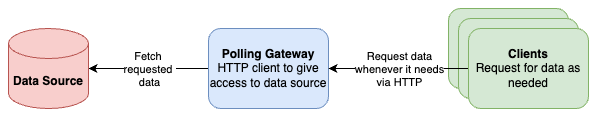
\includegraphics[width=1\textwidth]{Gateway-Pooling Gateway.drawio}
    \caption{Pooling Gateway Architecture.\label{fig:subfigures3}}
\end{figure}

\subsection*{Broadcaster gateway}
\label{sec:broadcaster}

In this scenario, the gateway provides a subscription service with asynchronous message sender API. Each consumer can subscribe to the gateway by registering its desired data and address, and the gateway notifies on triggers. These messages and subscription are made with HTTP requests. Note that the data provider needs some type of storage to keep track of the subscribed services. For this implementation, it uses a CSV file, but it could be any other most usual database. The base implementation is detailed at the pull request: https://github.com/gfmota/charging-plug-gateway/pull/6

\begin{figure}
    \centering
    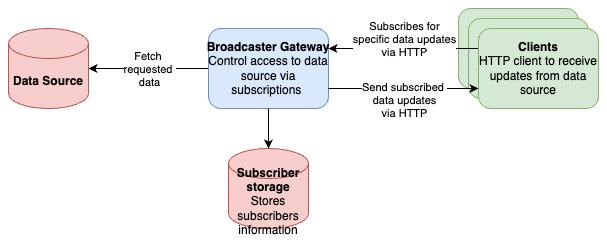
\includegraphics[width=1\textwidth]{Gateway-Broadcaster Gateway.drawio}
    \caption{Broadcaster Gateway Architecture.\label{fig:subfigures4}}
\end{figure}

{Message queue-based gateway}
\label{sec:messagequeue}

In this scenario, the data provider offers an asynchronous event-notifier API to provide data to the consumers. The data provider retrieves the data upon triggers and post it to a topic as a message with a tag that specifies the type of data it contains. Each data consumer is responsible for creating its own queue and attaching it to the topic with the correct message tag according to the data it wants. This implementation uses RabbitMQ, but it could be any other broker with topic implementation. The base implementation is detailed at the pull request: https://github.com/gfmota/charging-plug-gateway/pull/2

\begin{figure}
    \centering
    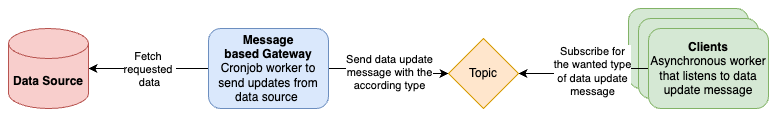
\includegraphics[width=1\textwidth]{Gateway-Message based Gateway.drawio}
    \caption{Message queue-based Gateway Architecture.\label{fig:subfigures5}}
\end{figure}

\section{Execution}
\label{sec:execution}

To run the experiment, it was created a repository with gateway and analyzer repositories, and scripts to run each scenario. https://github.com/gfmota/charging-plug-experiment

\begin{program}
    \index{Bash}
    \centering
  
  \begin{lstlisting}[language=bash, style=wider]
    ./run_polling_experiment.sh
  \end{lstlisting}
  
    \caption{Command to run polling scenario.\label{prog:java1}}
\end{program}

\begin{program}
    \index{Bash}
    \centering
  
  \begin{lstlisting}[language=bash, style=wider]
    ./run_broadcaster_experiment.sh
  \end{lstlisting}
  
    \caption{Command to run broadcaster scenario.\label{prog:java2}}
\end{program}

\begin{program}
    \index{Bash}
    \centering
  
  \begin{lstlisting}[language=bash, style=wider]
    ./run_message_experiment.sh
  \end{lstlisting}
  
    \caption{Command to run message based scenario.\label{prog:java3}}
\end{program}

All of them can receive an integer parameter to define the amount of clients the gateway will handle simultaneously, this doesn't mean that it will run n clients application, but a single application that will mimic n clients.

These scripts run the gateway and client application on ports 8080 and 8081 respectively, and also makes available metrics graphs on Grafana that you can access at port 3000 at /dashboard (login is admin/admin). These metrics are going to be used to evaluate how the gateway's performance behavior with multiple clients and different features.

There is also applications' log on /log to debug any unexpected behavior.

On polling experiment, instead of using the analyzer, it was replaced by jmeter, a load testing tool, highly configurable, that can simulate multiple HTTP clients requesting data at the same time.

\section{Results}
\label{sec:results}

The results contain the amount of changes necessary during the second development cycle and the Grafana's dashboards after multiple execution with different amount of clients to serve, 10, 100 and 1000..

Every board contains graphs of CPU and memory percentage usage by the application, and a graph with the amount of data access according to the Open Data Hub time of information: last status is used by current status feature, and time range is used by daily and hourly report.

\subsection*{Polling gateway}
\label{sec:pollingresult}

The code necessary to implement the new feature at the Polling gateway is at this PR https://github.com/gfmota/charging-plug-gateway/pull/5 (Figure~\ref{fig:pollingdif})

\begin{figure}
    \centering
    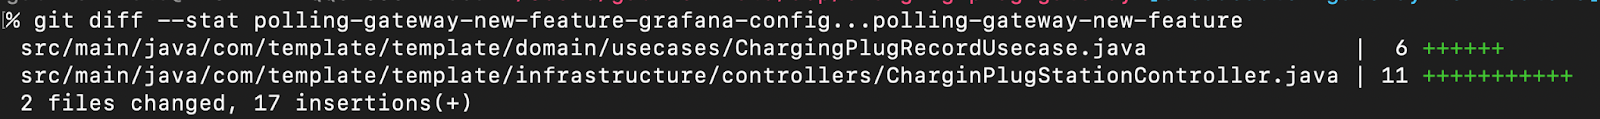
\includegraphics[width=1\textwidth]{pollingdif}
    \caption{Polling gateway extension code diff.\label{fig:pollingdif}}
\end{figure}

The execution of the experiment consists of a jmeter load test with 10, 100 and 1000 clients to simulate different clients at the same time.

\begin{figure}
    \centering
    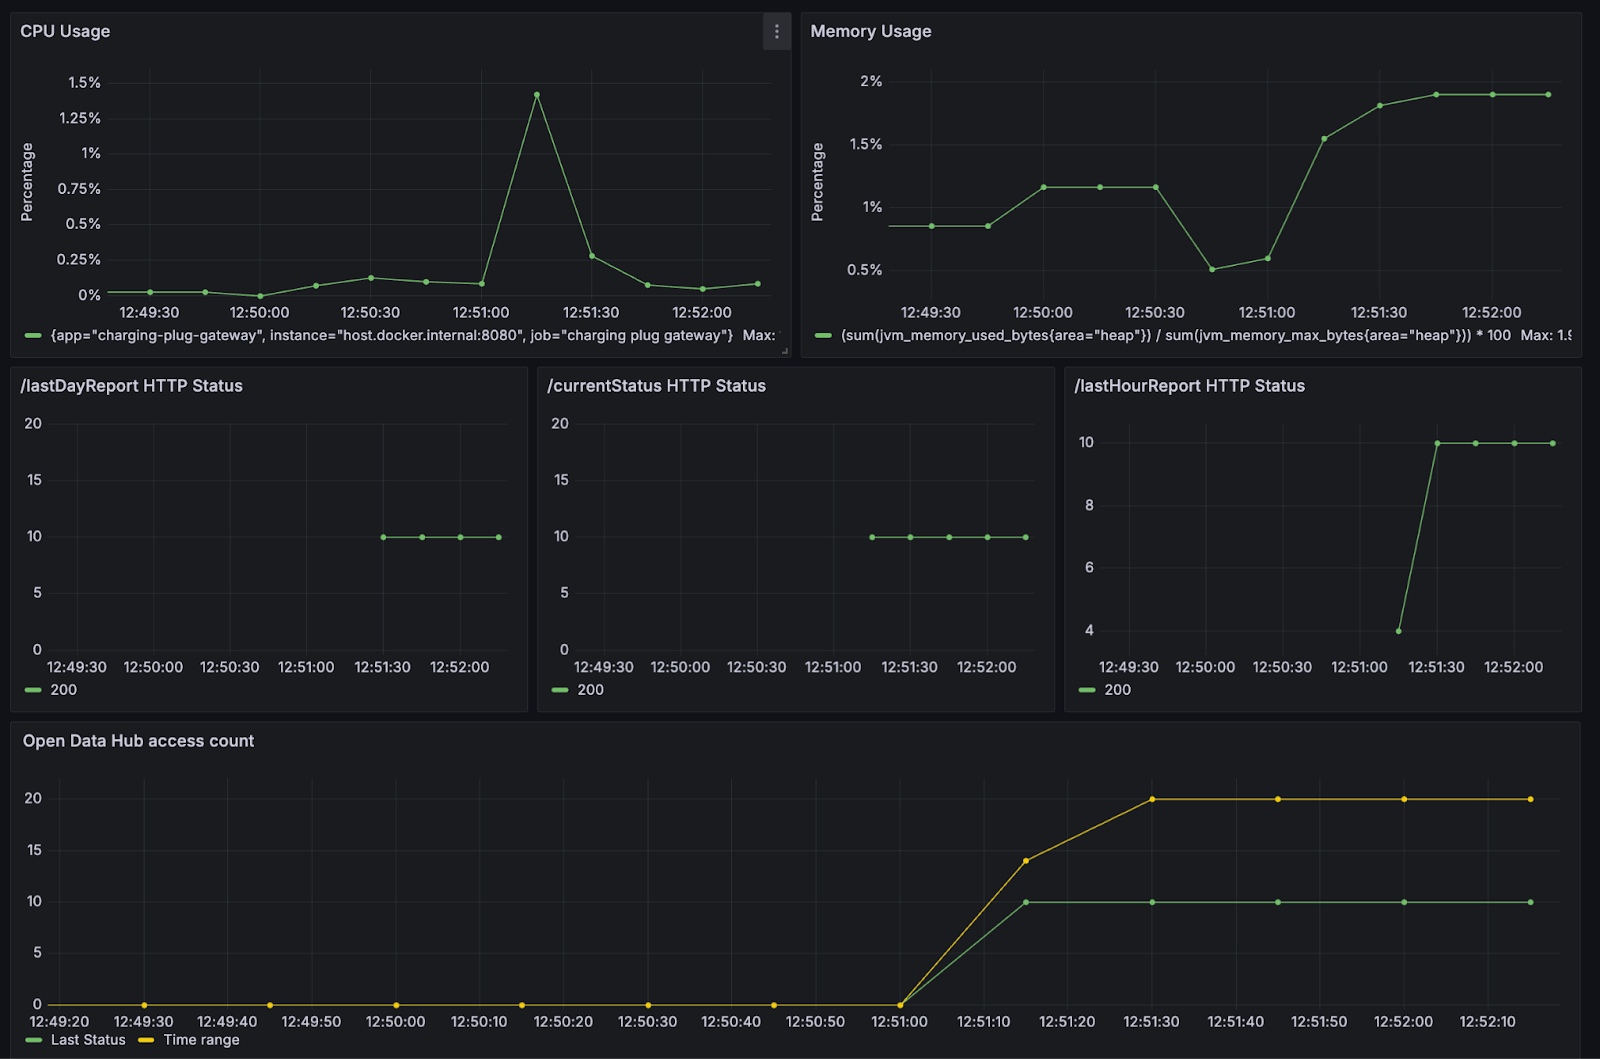
\includegraphics[width=1\textwidth]{polling10}
    \caption{Polling gateway experiment with 10 clients per feature runtime metrics.\label{fig:polling10}}
\end{figure}

In regards to figure~\ref{fig:polling10}: The first line contains charts of CPU and memory usage by the application during the experiment, notice that the CPU peaks on the moments the requests are received (12:51:00). On the second line, there are charts with the HTTP status of the response for each endpoint. In this case, the application was able to respond to all requests successfully, represented by the 200 OK status code. The third line contains a chart with the amount of data access made to the Open Data Hub, the data source, by the type of query. The current status feature uses the last status query, while last hour and last day report uses the time range query. For this reason, there is the double of time range queries made than the last status. 

\begin{figure}
    \centering
    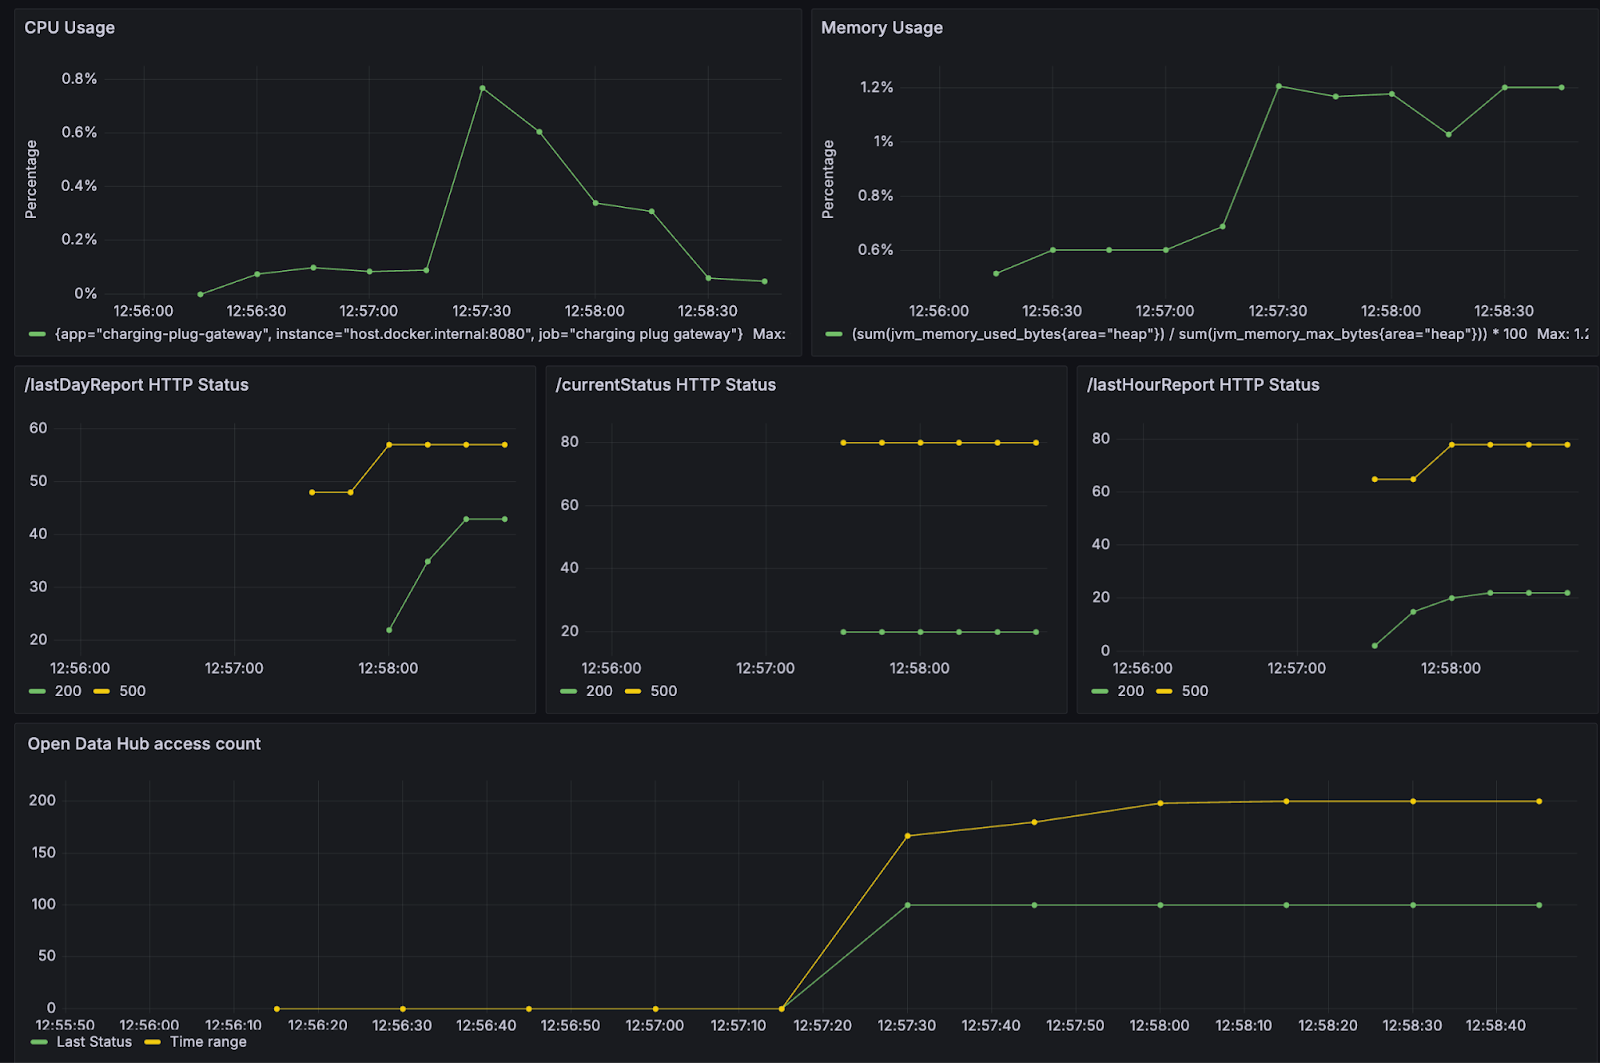
\includegraphics[width=1\textwidth]{polling100}
    \caption{Polling gateway experiment with 100 clients per feature runtime metrics.\label{fig:polling100}}
\end{figure}

In regards to figure~\ref{fig:polling100}: In this case, the data provider fails to respond around 70% of the clients, represented by the amount of 500 status code on the requests responses for each endpoint.

\begin{figure}
    \centering
    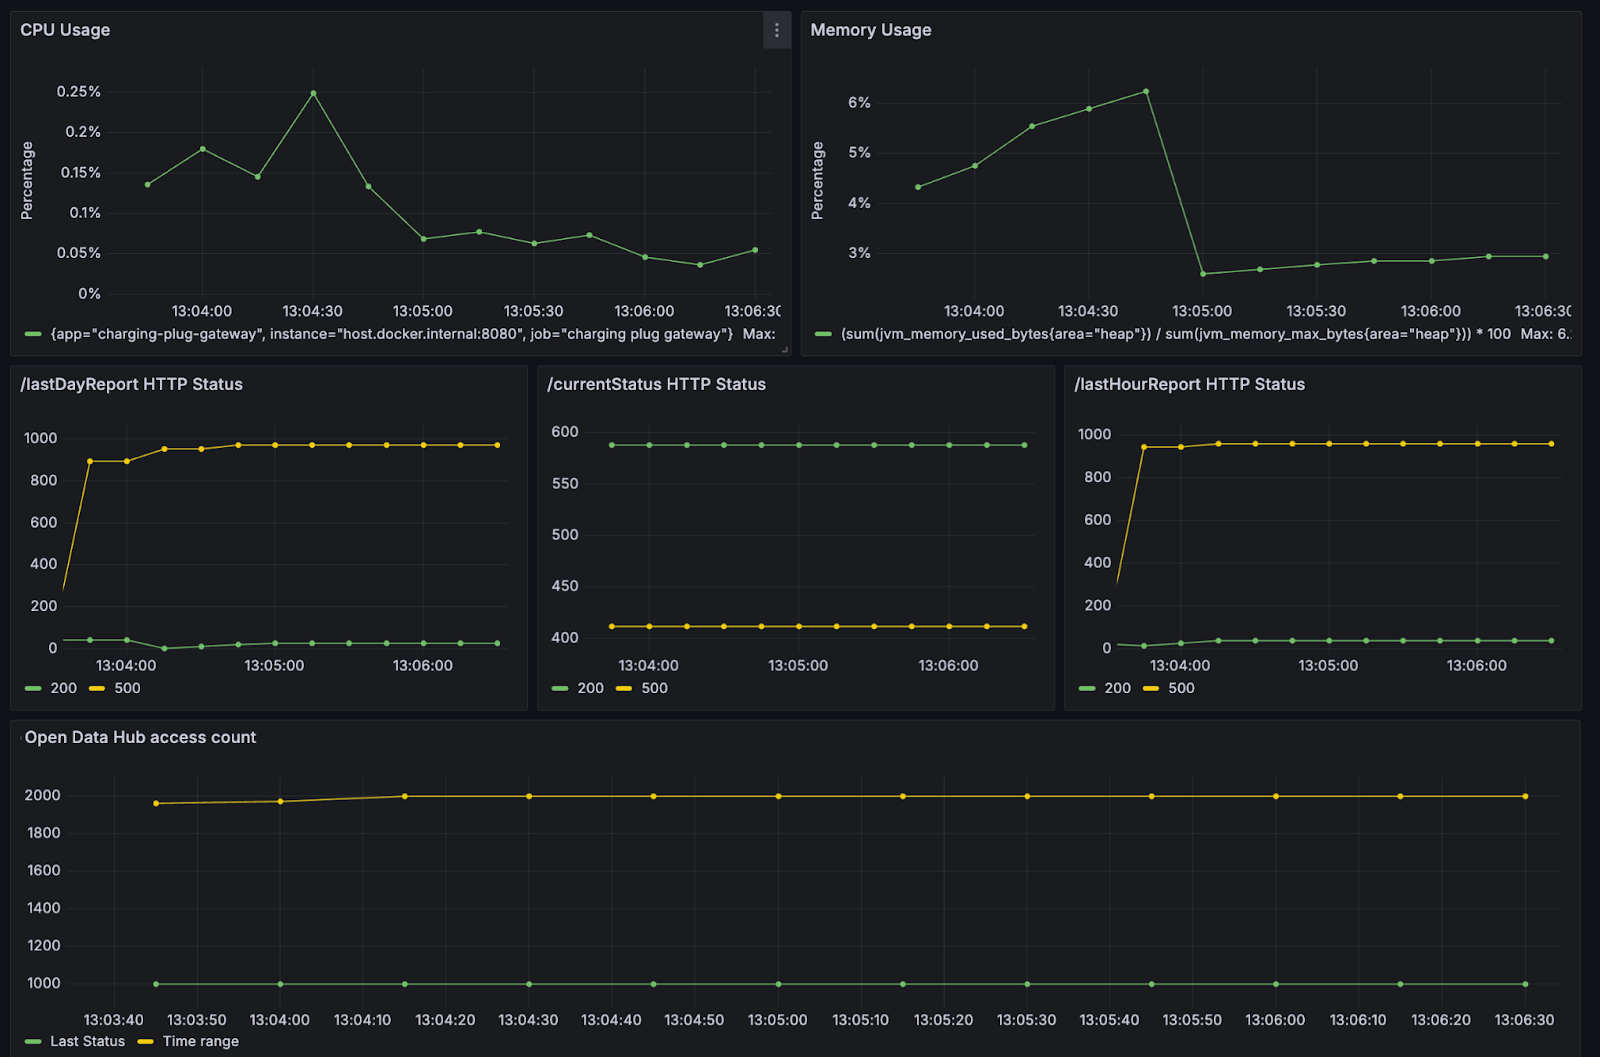
\includegraphics[width=1\textwidth]{polling1000}
    \caption{Polling gateway experiment with 1000 clients per feature runtime metrics.\label{fig:polling1000}}
\end{figure}

In regards to figure~\ref{fig:polling1000}: During this execution, the provider failed to respond to almost 80% of requests.

Notice that, in all executions, the CPU peaks during the requests handling. The memory usage tends to increase as the amount of requests increase and, consequently, the amount of objects to handle in memory. Also note that the amount of data lake access increases with the number of requests, since for each incoming request, the data gateway makes a new query on the data source.

\subsection*{Broadcaster gateway}
\label{sec:broadcasterresult}

The code necessary to implement the new feature at the Broadcaster gateway is at https://github.com/gfmota/charging-plug-gateway/pull/7 (Figure~\ref{fig:broadcasterdif})

\begin{figure}
    \centering
    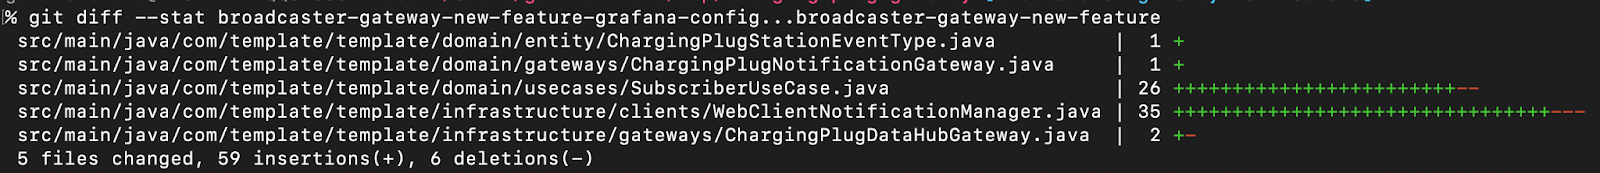
\includegraphics[width=1\textwidth]{broadcasterdif}
    \caption{Broadcaster gateway extension code diff.\label{fig:broadcasterdif}}
\end{figure}

The experiment consists of a client sending 10, 100 and 1000 requests per feature to the /subscribe endpoint at the gateway, subscribing itself to the gateway. Furthermore, on a CronJob trigger, it sends requests to every subscribed client with the requested data.

\begin{figure}
    \centering
    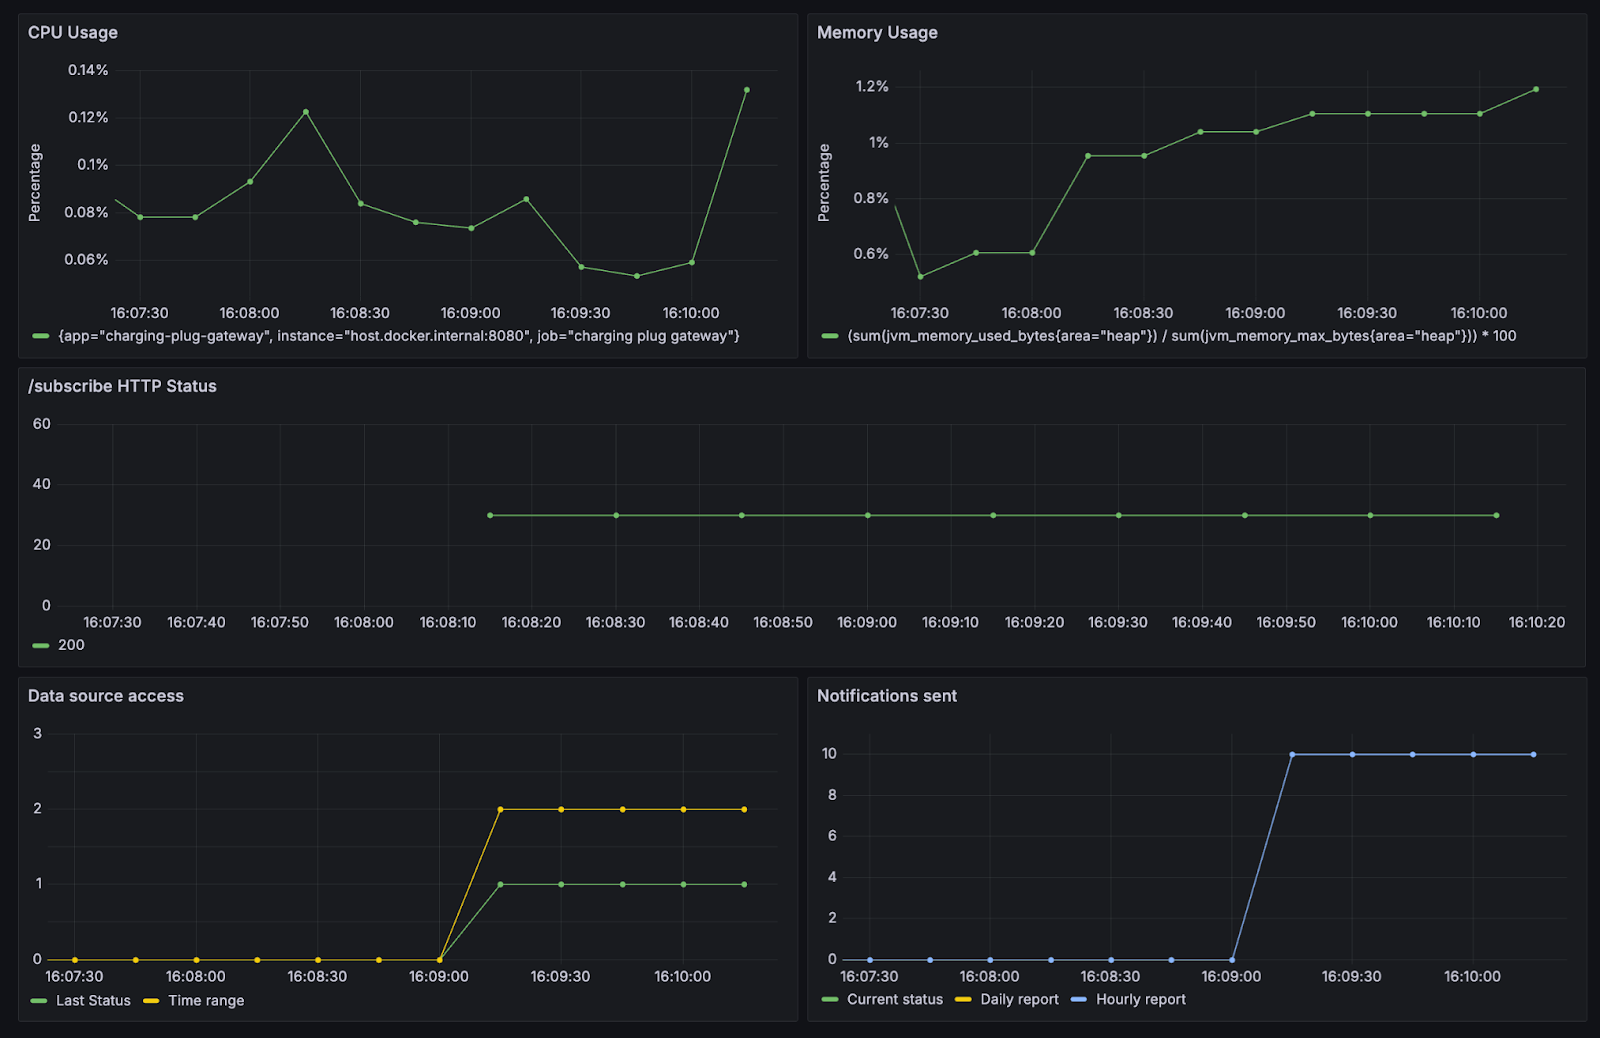
\includegraphics[width=1\textwidth]{broadcaster10}
    \caption{Broadcaster gateway experiment with 10 clients per feature runtime metrics.\label{fig:broadcaster10}}
\end{figure}

In regards to figure~\ref{fig:broadcaster10}: The first line is the same as in the previous scenario. The second line is a chart with the HTTP status of the response for the subscription endpoint. It shows there were 30 subscriptions, and on the next trigger, the notifications are sent for the services subscribed, as shown in the third line that contains charts for the data access made on Open DataHub and the amount of notifications sent for each type of data.

As the trigger was at the same moment for the three type of notifications, the lines on the notification sent chart overlapped, this means that the notifications were sent at the same moment and in the same amount.

In the last line the charts shows that no matter how many notifications are sent, it is required to retrieve data only once per type of notification, once in last status to notify the current status and two time range data access for hourly and daily notifications, as stated on the last scenario.

\begin{figure}
    \centering
    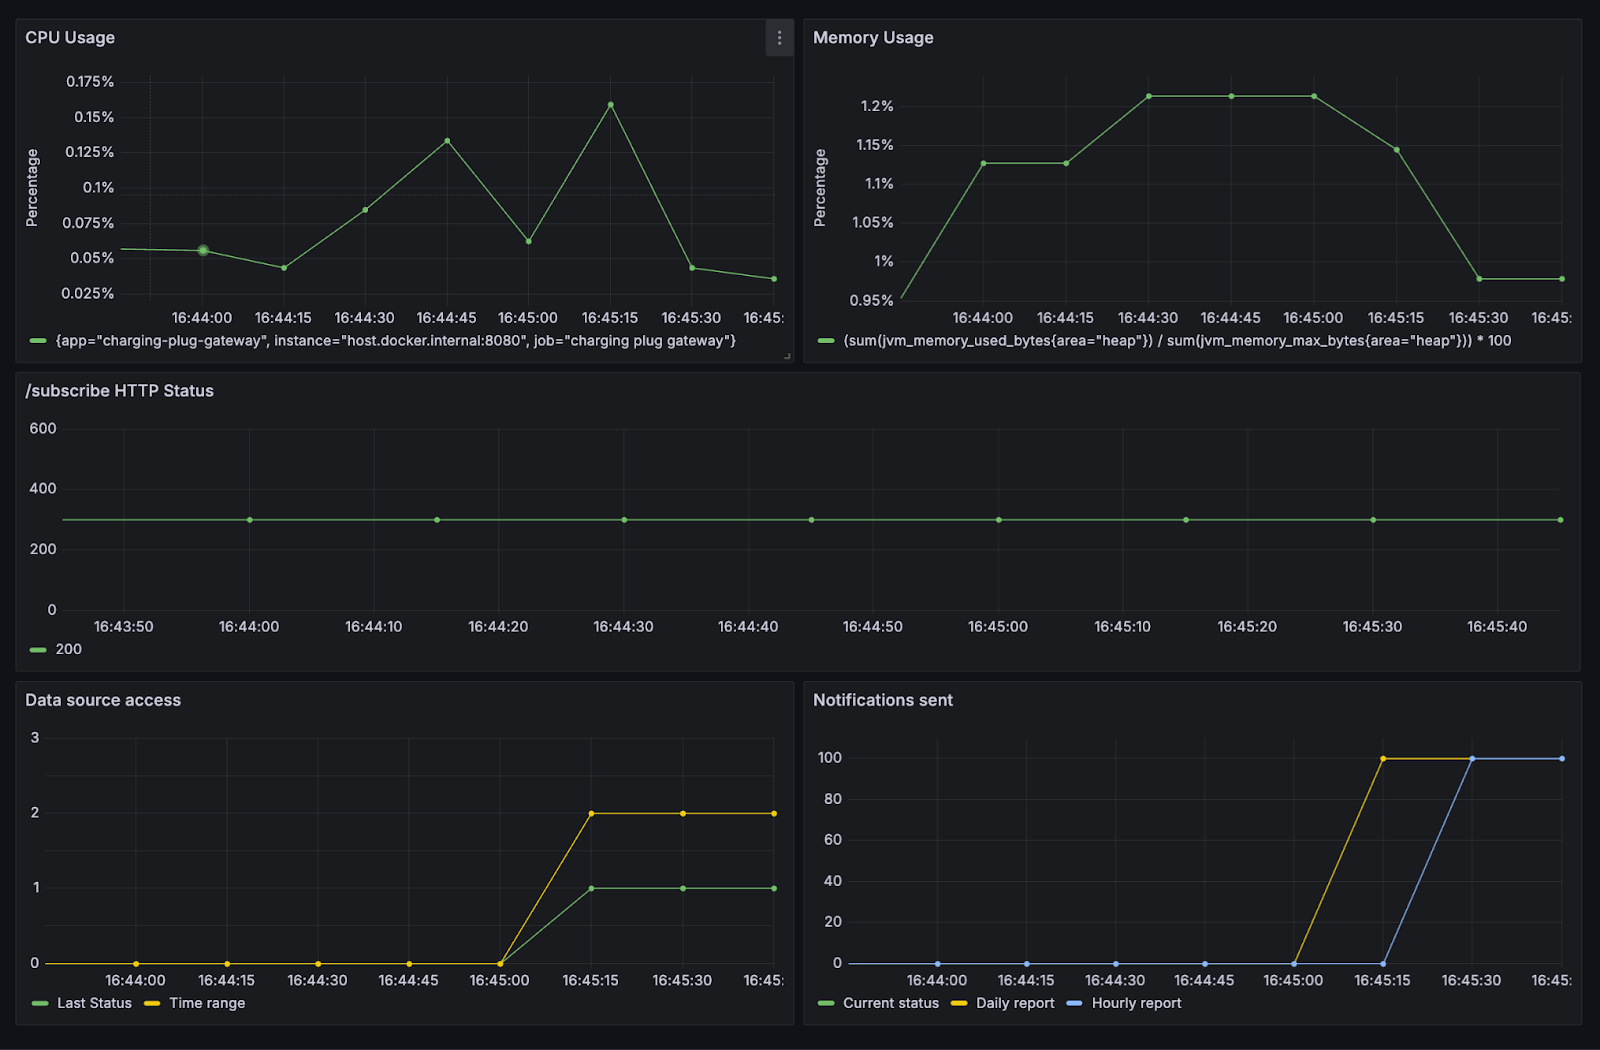
\includegraphics[width=1\textwidth]{broadcaster100}
    \caption{Broadcaster gateway experiment with 100 clients per feature runtime metrics.\label{fig:broadcaster100}}
\end{figure}

\begin{figure}
    \centering
    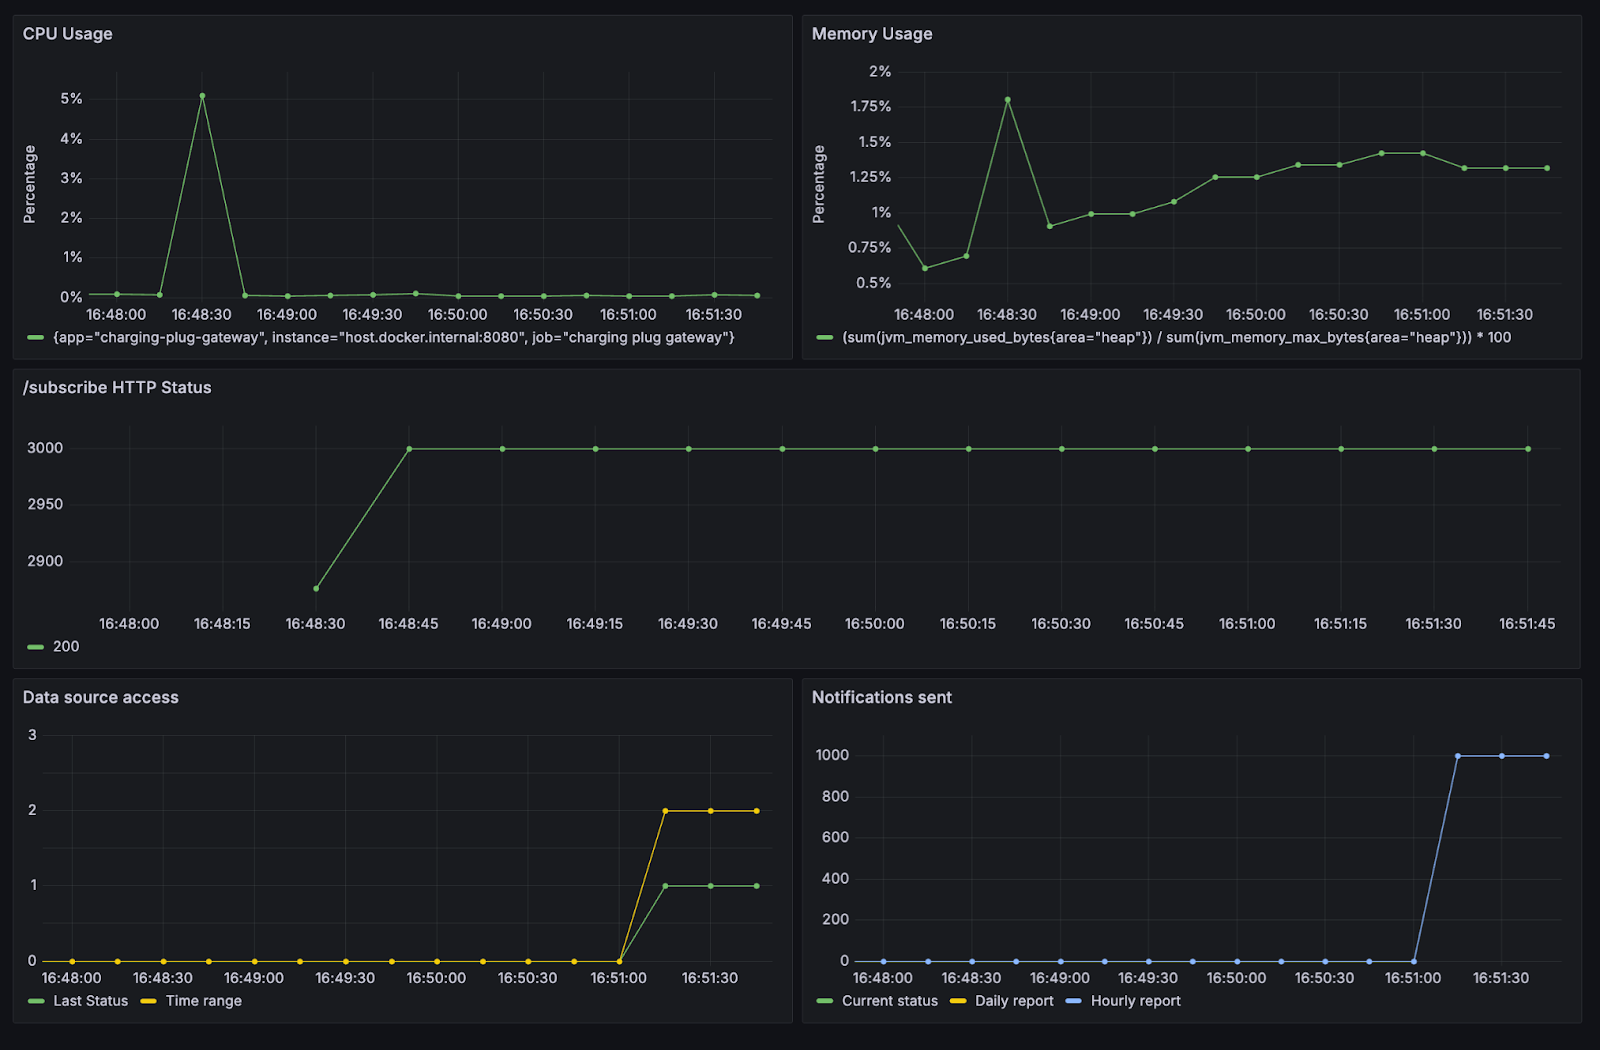
\includegraphics[width=1\textwidth]{broadcaster1000}
    \caption{Broadcaster gateway experiment with 1000 clients per feature runtime metrics.\label{fig:broadcaster1000}}
\end{figure}

In regards to figure~\ref{fig:broadcaster1000}: On this execution, it is possible to observe how the amount of notifications sent affect the application. The CPU and memory usage peaks as it receives a large amount of subscription requests, as happens in the first scenario with an HTTP handler. However, in this execution, the memory also peaks during notification, this happens because each notification requires an HTTP connection, each connection requires memory, this can be detrimental as the amount of notifications sent increases.

\subsection*{Message queue-based gateway}
\label{sec:messageresult}

The code necessary to implement the new feature at the Message queue-based gateway is at https://github.com/gfmota/charging-plug-gateway/pull/8 (Figure~\ref{fig:messagedif})

\begin{figure}
    \centering
    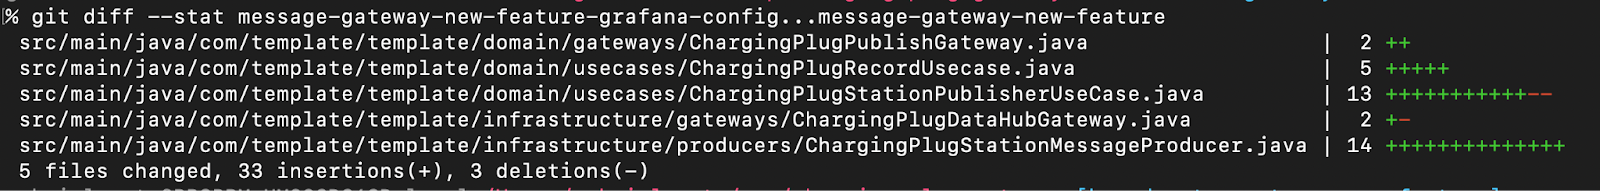
\includegraphics[width=1\textwidth]{messagedif}
    \caption{Message queue-based gateway extension code diff.\label{fig:messagedif}}
\end{figure}

The experiment consists of a client creating 10, 100 and 1000 queues per feature and attaching it to the topic created by the gateway. For each queue, the client creates a consumer to simulate multiple independent clients. On a CronJob trigger, the gateway sends a message per feature to the topic.

\begin{figure}
    \centering
    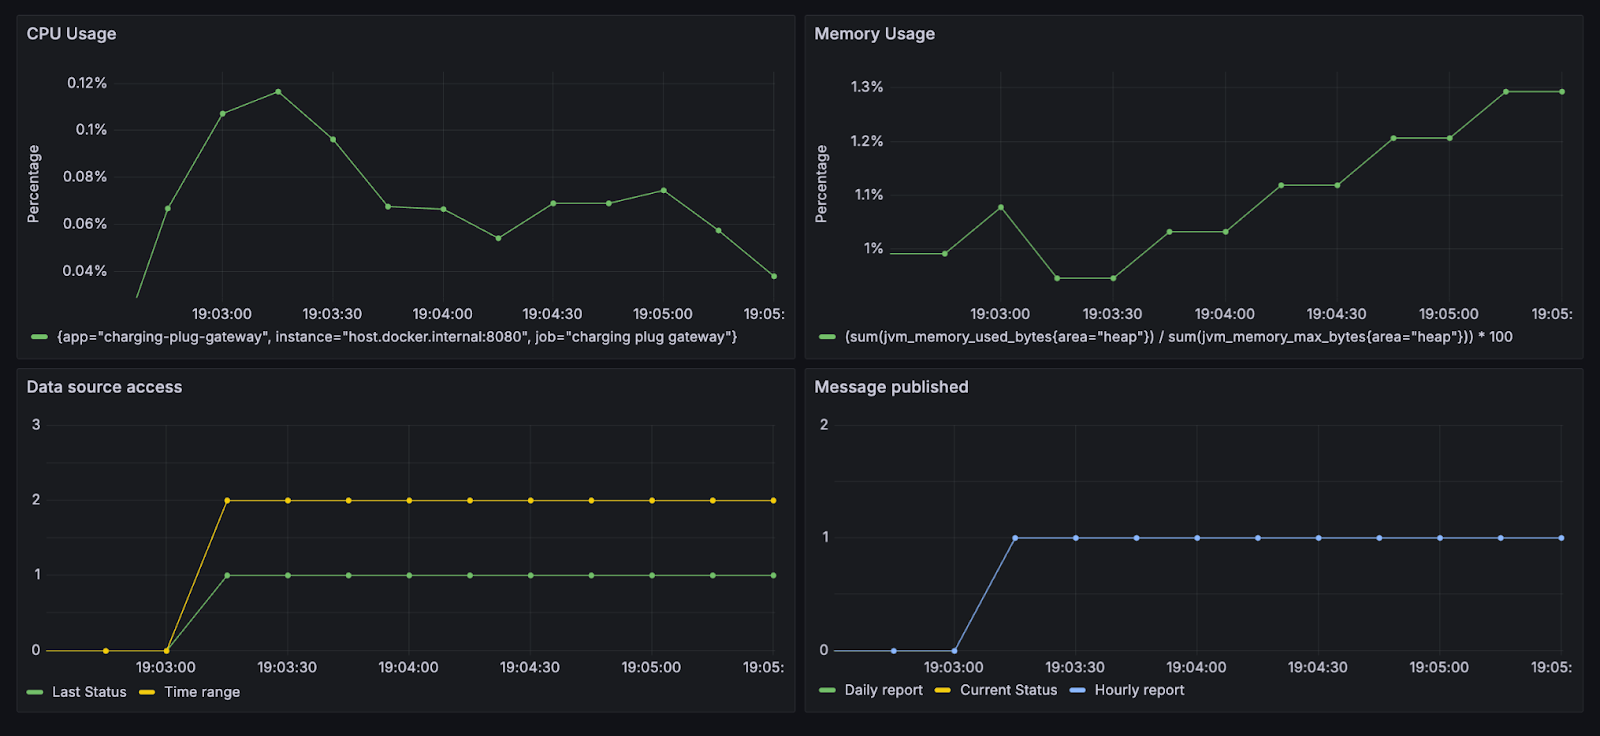
\includegraphics[width=1\textwidth]{message10}
    \caption{Message queue-based gateway experiment with 10 clients per feature runtime metrics.\label{fig:message10}}
\end{figure}

In regards to figure~\ref{fig:message10}: The first line contains are the same as described in the precious scenarios. In the second line, there is a chart of the amount of data access to source per type of data queried, remembering that daily and hourly features requires access to time range data and current status requires access to last status data. There is also a chart with the amount of messages published per type of message or feature. As happened in the previous scenario, the messages are sent at the same time, for this reason the lines in the chart may overlap.

\begin{figure}
    \centering
    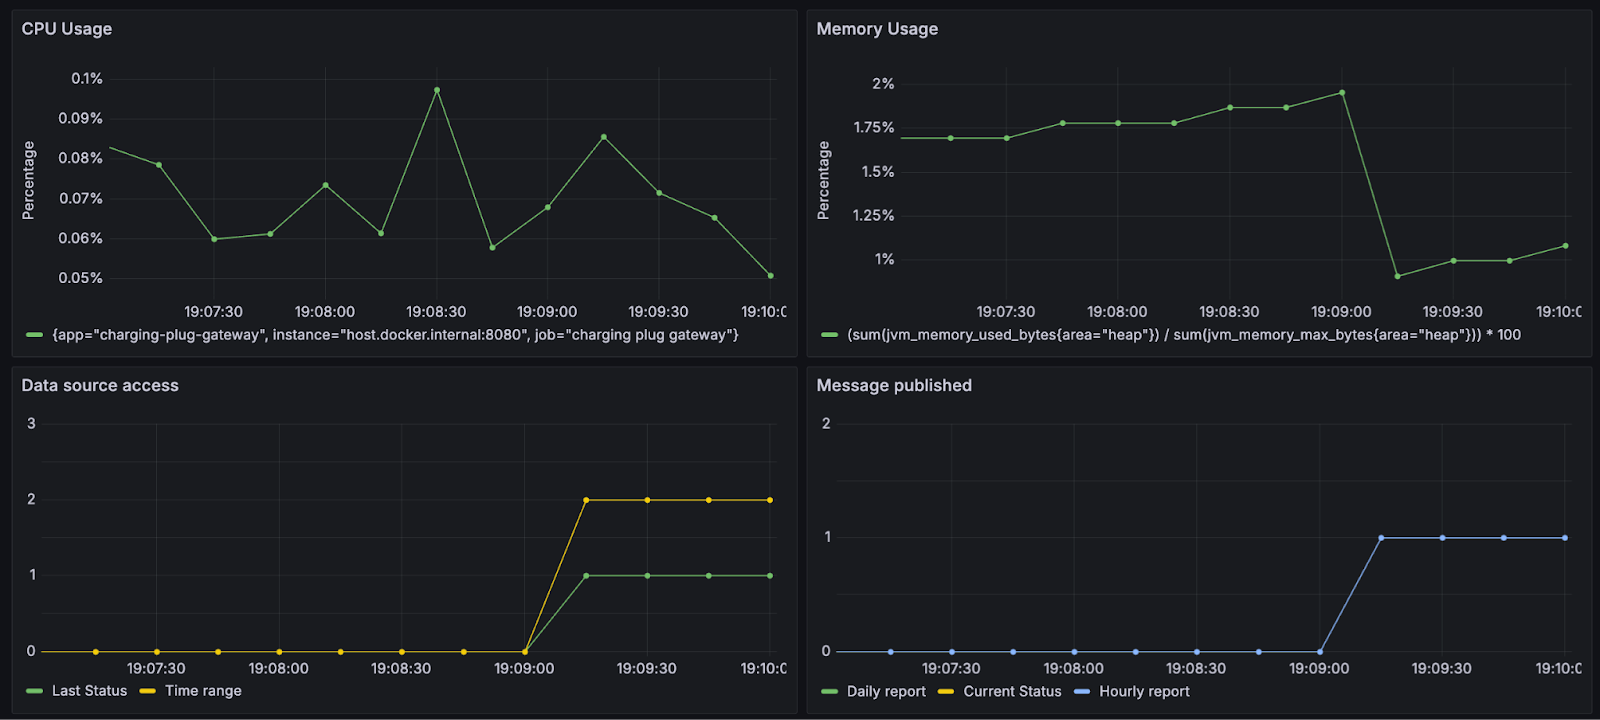
\includegraphics[width=1\textwidth]{message100}
    \caption{Message queue-based gateway experiment with 100 clients per feature runtime metrics.\label{fig:message100}}
\end{figure}

\begin{figure}
    \centering
    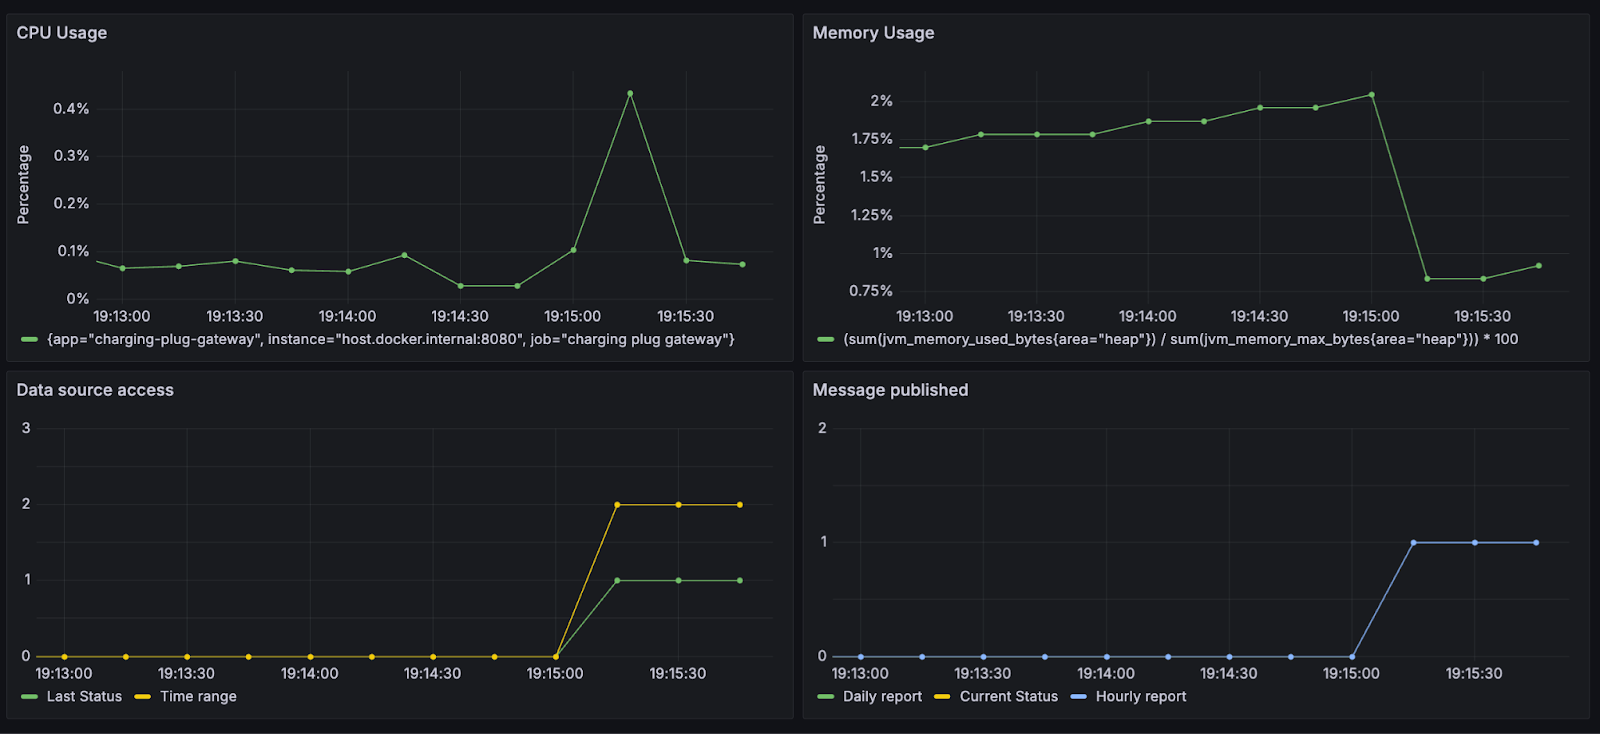
\includegraphics[width=1\textwidth]{message1000}
    \caption{Message queue-based gateway experiment with 1000 clients per feature runtime metrics.\label{fig:message1000}}
\end{figure}

Notice that, as in the Broadcaster, there is only one data source access per feature per trigger, however, for each trigger, only one message is sent per feature, no matter how many data consumers are served. This also means that the CPU and memory usage is close to equal for all executions.

\section{Takeaways}
\label{sec:providerconclusion}

After the experiments, it's possible to take some conclusions about each scenario according to extensibility.

\subsection*{Extensibility and Development experience}
\label{sec:devex}

When looking for number of code changes at the git diff for each scenario, the Polling Gateway had the least line changes for the base implementation and for feature addition.

However, all have similar work necessary to add new features, and the base implementation depends on how comfortable the developer is with the infrastructure used. On the perspective of a junior developer, synchronous communication with HTTP can be easier, since it is more common and thus used a base concept for multiple subjects, such as web development. While message broker and asynchronous communication are advanced concepts and require more complex tools and knowledge, what can end up intimidating these developers.

\subsection*{Data source usage}
\label{sec:source}

The chart of data source accesses shows that the Broadcaster and Message queue-based gateway use a constant number of data access independent of the number of clients. Meanwhile, the Polling gateway has to access the data source every time it receives a request, even thought the result hasn’t changed.

This characteristic of the polling gateway can be detrimental to the application environment since each request depends on I/O, adding response time, and leading to unnecessary computation by the data source service.

To minimize these, it is possible to use cache on data source calls. On the experiment use case, it was necessary to implement an in-memory cache, due to the data source being a third-party open API. 

However, the in-memory cache is not recommended in all cases, for example in big applications, where it is likely to have multiple Pods running the same application, each Pod has its own memory and can't share it with others. Therefore, in-memory cache wouldn't be 100% effective and can be replaced by a more robust solution. There are different types of caches and the choice depends on the effective needed and the budget available for infrastructure solutions.

Using cache would also imply on the infrastructure cost increase. The cost can vary depending on the tool, it can be cheap as in-memory cache, or higher using a fast access database.

\subsection*{Scalability}
\label{sec:scala}

Scalability is used in regard to how well each scenario deals with the increase of clients. At first, the Polling gateway seems the least scalable, with the client number increase, it started to have fail to deal with the requests and throwing error to clients. It means that clients of the Polling gateway needs to have some fallback mechanisms, like retry implementation.

It is possible to minimize it by adding horizontal scaling and load balancing, doing so would be able to distribute requests and thus processing required. However, this would require an increase in cost and in infrastructure complexity.

Due to the nature of the Broadcaster gateway to only send requests from time to time, with a cron job or observing updates on the data source, it has low CPU usage for most of the time. However, when it starts the process to notify the subscribed clients, the CPU usages increase according to the number of clients, since each one needs a request.

There are also considerations about the subscription method. The subscribe endpoint can end up having  problems with availability if it receives a big volume of requests at the same time, as in the Polling gateway. Even thought, this endpoint is not planned to have high usage, there should be worry about how to deal with lost requests.

It is also important to have safe unsubscribe methods. It can help avoid sending unnecessary requests and thus saving CPU usage.

While the Message queue-based gateway have the same behavior of the Broadcaster according to when it sends data to clients, it doesn't peak CPU usage during processing data and publishing messages, thus can be said the best solution to scale. This is because the gateway have constant processing no matter how many clients it is serving, since it can serve multiple clients with a single message.

\subsection*{Client autonomy}
\label{sec:client}

Another point to take in consideration when comparing each scenario, is how much each client is attached to the gateway solution. The Broadcaster experiment have an example of an attached client.

The Broadcaster's client needs to have an HTTP endpoint available all the time for gateway updates. For this reason, it is important to the Broadcaster gateway to add a failure mechanism, such as retry implementation, in case the client is unavailable or with high traffic.

\begin{figure}
    \centering
    \includegraphics[width=.8\textwidth]{Gateway-Página-3.drawio}
    \caption{Broadcaster gateway dependency diagram.\label{fig:subfigures6}}
\end{figure}

The Polling gateway shows what a bad autonomy is. The client is autonomous to request the data it wants whenever it needs. It can save CPU usage sometimes, since, if there is no request, there is no need for the gateway to retrieve data and process it. However, as it is the client's responsibility to request the data, there is no way for the client to know if there is a data update. This can cause the client to request multiple times for the same data, wasting both gateway and client processing capability with repeated data.

\begin{figure}
    \centering
    \includegraphics[width=.8\textwidth]{Gateway-Página-2.drawio}
    \caption{Polling gateway dependency diagram.\label{fig:subfigures7}}
\end{figure}

While the Message queue-based gateway have the best example of autonomy. The client service does not need to be available for the gateway, since the queue can store the messages until they are consumed. The client can also consume the data from the queue whenever it wants, but only if it is an update available, otherwise there will be no message on the queue, avoiding consuming repeated data as in the Polling scenario.

\begin{figure}
    \centering
    \includegraphics[width=.8\textwidth]{Gateway-Página-4.drawio}
    \caption{Message queue-based gateway dependency diagram.\label{fig:subfigures8}}
\end{figure}

\subsection*{Infrastructure cost}
\label{sec:infra}

Each scenario have its own environment and needs. As in a software system, it is important to consider the cost in regard to all services used by an application, each service requires maintenance and have a cost attached to it.

In this regard, the Polling gateway may seen ahead because in the first implementation there is no need of extra services to support it. However, as discussed previously, this is not true when scalability is necessary, requiring cache tools and horizontal scaling to perform well on high usage scenarios.

The Broadcaster gateway requires only a database to store the clients subscribed to the service. For this reason, it is important to create routines to keep the data clean of unused information and a good indexing to minimize IO time. It is important to note, as mentioned previously, for each notification sent it is necessary to create a new HTTP connection, connections use network bandwidth, this can become a problem as the amount of clients increase and cause increasing cloud cost as the bandwidth used get larger.

The Message queue-based requires a message broker for the implementation, but also is the only one that requires a message broker on the client side. This can be trick when dealing with multisource clients, depending on the use case.
